% -*- TeX:de -*-
\NeedsTeXFormat{LaTeX2e}
\documentclass[12pt,a4paper,titlepage]{article}

%\usepackage[german]{babel} % german text
\usepackage[DIV12]{typearea} % size of printable area
\usepackage[T1]{fontenc} % font encoding
\usepackage[utf8]{inputenc} % probably on Linux

\usepackage{graphicx} % to include images
\graphicspath{ {img/} } % set default image directory
\usepackage{subfigure} % for creating subfigures
\usepackage{amsmath} % a bunch of symbols
\usepackage{amssymb} % even more symbols
\usepackage{booktabs} % pretty tables
\usepackage{csquotes}

% a floating environment for circuits
\usepackage{float}
\usepackage{caption}

\newfloat{circuit}{tbph}{circuits}
\floatname{circuit}{Schaltplan}

% a floating environment for diagrams
\newfloat{diagram}{tbph}{diagrams}
\floatname{diagram}{Diagramm}

\renewcommand{\familydefault}{\sfdefault} % activate to use sans-serif font as default

\sloppy % friendly typesetting

\usepackage{eurosym}
\usepackage{makeidx}
\usepackage{amsfonts}
\usepackage{mparhack}
\usepackage{array}
\usepackage{tabularx}
\usepackage{minitoc}
\usepackage[colorlinks=true]{hyperref}
\usepackage{epstopdf}
\usepackage{setspace}
\usepackage{csquotes}
\usepackage{circuitikz}

% hyperref settings
\hypersetup{
    colorlinks=false,       % false: boxed links; true: colored links
    linkcolor=black,          % color of internal links (change box color with linkbordercolor)
    citecolor=black,        % color of links to bibliography
    filecolor=black,      % color of file links
    urlcolor=black           % color of external links
}

\begin{document}

\begin{titlepage}

\begin{figure*}[h!]
  
\includegraphics[width=8cm]{TULogo_CMYK}
\end{figure*}

\begin{center}
\vspace*{1.3cm}
{\Huge Elektrotechnische Grundlagen der Informatik\\(LU 182.692)\\}
\vspace{1.7cm}
{\LARGE Protokoll der 2. Labor\"ubung: \enquote{Filter}\\}
{\large \enquote{Transiente Vorg\"ange und Frequenzverhalten}\\}
{\LARGE b) Messungen\\}
\vspace{1.5cm}

% fill in group number and date of lab here
% CHANGE ME!
{\Large Gruppennr.: 22 \hspace{1cm} Datum der Labor\"ubung: 19.05.2017}

% fill in IDs and names here
% CHANGE ME!
\begin{table}[h!]
\centering
\begin{tabular}{|p{3.5cm}|p{3.5cm}|p{6.5cm}|}
\hline \textbf{Matr. Nr.} & \textbf{Kennzahl} & \textbf{Name} \\
\hline
1614835 & 033 535 & Jan Nausner \\
\hline
1633068 & 033 535 & David Pernerstorfer \\
\hline
\end{tabular}
\end{table}

\end{center}
\vspace{1.0cm}

\begin{table}[h!]
\begin{tabular}{|l|l|}
\hline \textbf{Kontrolle} & \checkmark \\
\hline Verhalten eines Filters 1. Ordnung & \\
\hline Verhalten eines RL-Filters & \\
\hline Dynamisches System 2. Ordnung & \\
\hline
\end{tabular}
\end{table}

\end{titlepage}
% start of actual lab protocol
% CHANGE ME!

\setcounter{page}{2}

\newpage
\setcounter{tocdepth}{1}
\tableofcontents

\newpage

\section*{Materialien}
\begin{itemize}
	\item Oszilloskop: Agilent InfiniiVision MSO-X 3054A
	\item Frequenzgenerator: Agilent 33220A
  \item Multimeter: Amprobe 37XR-A
\end{itemize}

\section{Messung des Verhaltens eines RC-Filters 1. Ordnung}

\subsection{Aufgabenstellung}
Die charakteristischen Eigenschaften eines RC-Tiefpassfilters mit realen Bauteilen sollen untersucht werden.

\subsection{Schaltplan}
\begin{figure}[H]
\centering
\begin{circuitikz}[european]
  \draw
    (0,2) to [R, l=$R$, o-] (3,2);
  \draw
    (3,2) to [short, *-o] (4,2);
  \draw
    (3,2) to [C, l=$C$] (3,0);
  \draw
    (0,0) to [short, o-o] (4,0);
\end{circuitikz}
\caption{RC Tiefpassfilter 1.Ordnung}
\label{Figure01}
\end{figure}


\subsection{Durchf\"uhrung}
Die Schaltung wurde gem\"a\ss\, Schaltplan mit einem Widerstand $R=22k\Omega$ und einem Kondensator $C=10nF$ aufgebaut. Um die Sprungantwort aufzuzeichnen wurde am Eingang ein periodisches Rechtecksignal mit $1 V_{PP}$, Offset $0,5 V$, $50 \%$ Duty Circle und Frequenz $250 Hz$, angelegt. Die Eingangs- und Ausgangsspannung wurden mit dem Oszilloskop im Zeitbereich aufgezeichnet (siehe Abbildung~\ref{Figure02}). Die Zeitkonstante wurde mit den gemessenen Bauteilwerten ($R=21,75 k\Omega$, $C=10,28nF$) berechnet und ergibt einen Wert von $\tau = RC = 226,16 \mu s$. Die Zeitkonstante wurde aus der Sprungantwort ausgelesen indem der Zeitpunkt gemessen wurde, an dem das Signal der Sprungantwort $632,75 mV$ (entspricht zirka $63 \%$ der Eingangsspannung) betrug (Vergleich siehe Tabelle ~\ref{Figure03}). \\
Am Eingang wurde nun ein Sinussignal mit $1 V_{PP}$, Offset $0 V$ angelegt. Die Eingangs- und Ausgangsspannung bzw. die Phasenverschiebung wurden mit dem Oszilloskop gemessen. Der Frequenzbereich von $10Hz$ bis $1MHz$ mit 5 Frequenzmesspunkten pro Dekade wurden abgetastet. Weiters wurde ein Frequenzmesspunkt an der Grenzfrequenz gesetzt. Die Messpunkte wurden in tabellarischer Form aufgezeichnet und in ein doppelt logarithmisches Diagramm eingetragen (siehe Abbildung~\ref{Figure04}). Ab der Frequenz von rund $20kHz$ konnte die Phasenverschiebung nicht mehr gemessen werden, da der Messwert am Oszilloskop sehr schwach war und dadurch zu stark schwankte.

\subsection{Ergebnis \& Diskussion}
\begin{figure}[H]
  \centering
  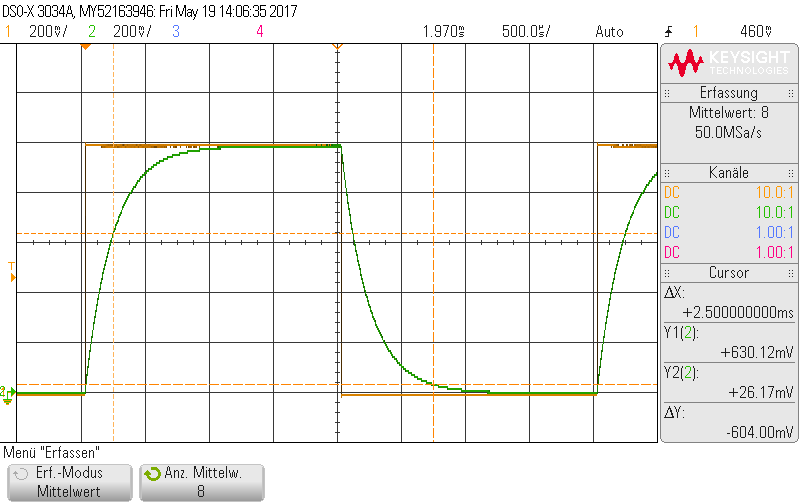
\includegraphics[width=100mm]{sprungantwort_rc_tiefpass.png}
  \caption{Sprungantwort RC Tiefpass}
  \label{Figure02}
\end{figure}
\noindent Die Sprungantwort der RC-Filterschaltung l\"asst auf einen Tiefpass 1.Ordnung schlie\ss en, da bei niedriger Frequenz die D\"ampfung $0dB$ ist und bei hoher Frequenz eine starke D\"ampfung zu erkennen ist.

\begin{table}[H]
  \centering
  \begin{tabular}{|c|c|c|c|}
  \hline
                     & berechnet    & gemessen    & Abweichung \\ \hline
  Zeitkonstante $\tau$ & $226,16 \mu s$    & $230 \mu s$      & $+1,70 \%$ \\ \hline
  \end{tabular}
  \caption{Vergleich Zeitkonstante $\tau$ berechnet und bemessen}
  \label{Figure03}
\end{table}
\noindent Die Zeitkonstante $\tau$ wurde bei einem Spannungswert von $632,75 mV$ ($63 \%$ der Eingangsspannung) gemessen und betr\"agt $230 \mu s$. Die Abweichung von $+1,70 \%$ kommt daher, dass es sich um reale Bauteile handelt.

\begin{figure}[H]
  \centering
  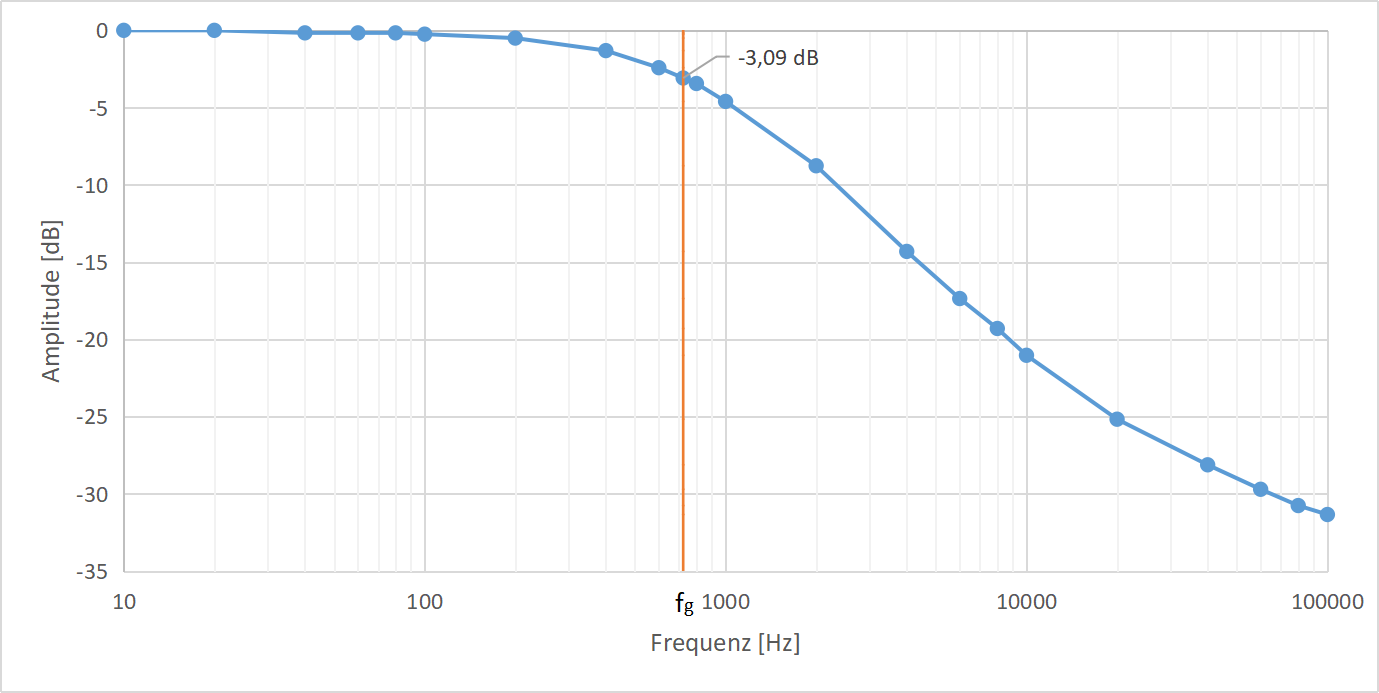
\includegraphics[width=100mm]{amplitudengang_rc_tiefpass.png}
  \caption{Amplitudengang RC-Tiefpass durch Messungen}
  \label{Figure04}
\end{figure}
\begin{figure}[H]
  \centering
  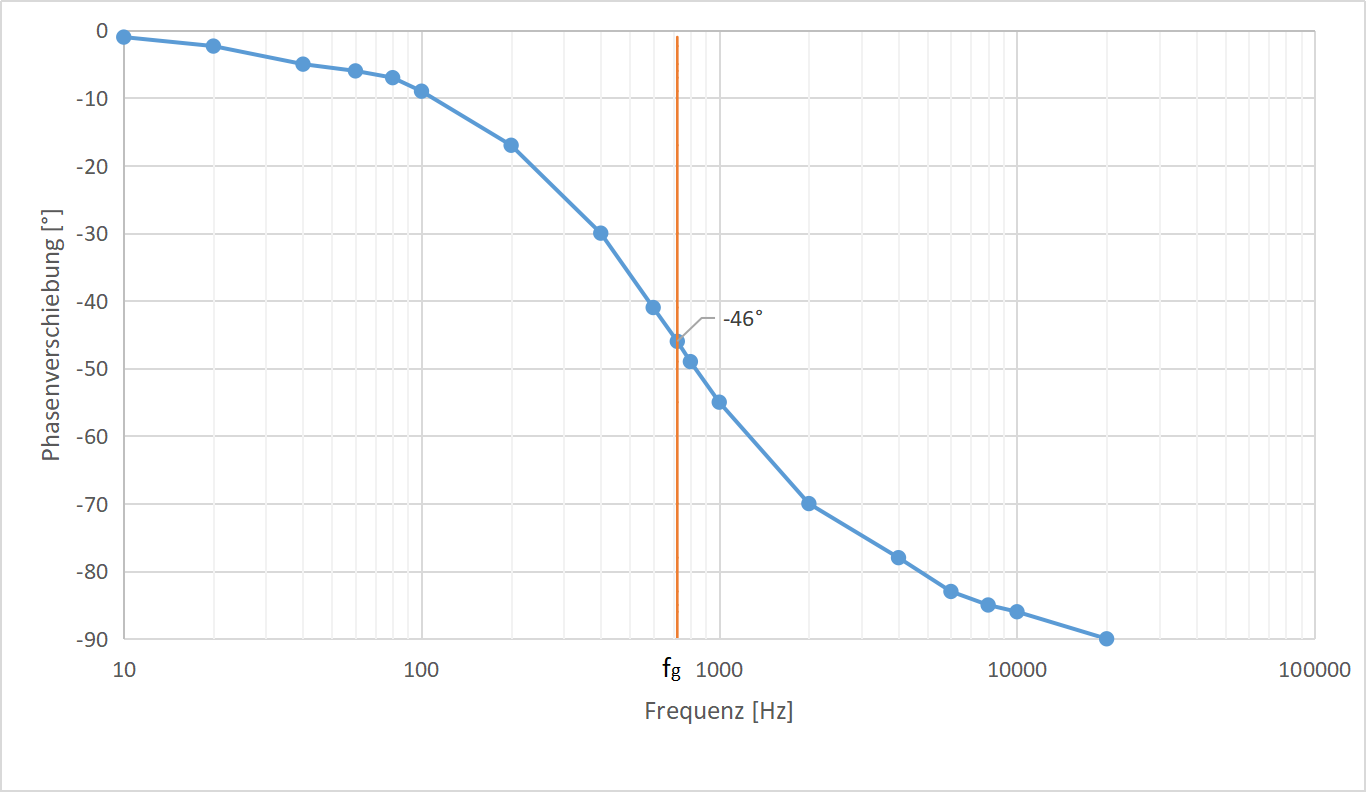
\includegraphics[width=100mm]{phasengang_rc_tiefpass.png}
  \caption{Phasengang RC-Tiefpass durch Messungen}
  \label{Figure05}
\end{figure}
In Abbildung~\ref{Figure04} und Abbildung~\ref{Figure05} sind Amplituden- und Phasengang des RC-Tiefpassfilters anhand der gemessenen Werte dargestellt. Der Graph entspricht der erwarteten Form aus der Simulation. Bei der Grenzfrequenz ($723Hz$) wurde am Ausgang eine Spannung von $750mV$ und eine Phasenverschiebung von $-46^{\circ}$ gemessen. Diese Werte sind plausibel, da lt. Berechnung und Simulation die Ausgangsspannung $\frac{1V}{\sqrt{2}} \approx 707,11mV$ und die Phasenverschiebung $-45^{\circ}$ sind. Bis zur Frequenz von rund $10kHz$ hat der Amplitudengang, wie erwartet, eine Filtersteilheit von $-20db/Dekade$. Bei idealen Bauteilen w\"are der Spannungswert ab einer gewissen Frequenz $0 V$. Bei realen Bauteilen jedoch wird diese D\"ampfung ($0V$) nie erreicht, stattdessen geht die D\"ampfung, wie in Abbildung~\ref{Figure04} zu erkennen, asymptotisch gegen $0V$.




\section{Messung des Verhaltens eines RL-Filters 1. Ordnung}

\subsection{Aufgabenstellung}

\subsection{Schaltplan}
\begin{figure}[H]
\centering
\begin{circuitikz}[european]
  \draw
    (0,2) to [R, l=$R$, o-] (3,2);
  \draw
    (3,2) to [short, *-o] (4,2);
  \draw
    (3,2) to [L, l=$L$] (3,0);
  \draw
    (0,0) to [short, o-o] (4,0);
\end{circuitikz}
\caption{RL Hochpassfilter 1.Ordnung}
\label{Figure06}
\end{figure}

\subsection{Durchf\"uhrung}
Die Schaltung wurde gem\"a\ss Schaltplan mit einem Widerstand $R=47\Omega$ und einem Kondensator $L=1mH$ aufgebaut. Um die Sprungantwort aufzuzeichnen wurde am Eingang ein periodisches Rechtecksignal mit $1 V_{PP}$, Offset $0,5 V$, $50 \% Duty Circle$ und Frequenz $2,5 kHz$, angelegt. Die Eingangs- und Ausgangsspannung wurden mit dem Oszilloskop im Zeitbereich aufgezeichnet (siehe Abbildung~\ref{Figure07}). Die Zeitkonstante wurde mit den gemessenen Bauteilwerten ($R=46,83 k\Omega$, $C=1,075mH$) berechnet und ergibt einen Wert von $\tau = \frac{L}{R} = 22,96 \mu s$. Die Zeitkonstante wurde aus der Sprungantwort ausgelesen indem der Zeitpunkt gemessen wurde, an dem das Signal der Sprungantwort $37 \%$ der Eingangsspannung betrug. \\
Am Eingang wurde nun ein Sinussignal mit $1 V_{PP}$, Offset $0 V$ angelegt. Die Eingangs- und Ausgangsspannung bzw. die Phasenverschiebung wurden mit dem Oszilloskop gemessen. Der Frequenzbereich von $10Hz$ bis $1MHz$ wurde mit 5 Frequenzmesspunkten pro Dekade abgetastet. Weiters wurde ein Frequenzmesspunkt an der Grenzfrequenz gesetzt. Die Messpunkte wurden in tabellarischer Form aufgezeichnet und in eine doppelt logarithmischen Diagrammm eingetragen (siehe Abbildung~\ref{Figure08} und Abbildung~\ref{Figure09}).

\subsection{Ergebnis \& Diskussion}
\begin{figure}[H]
  \centering
  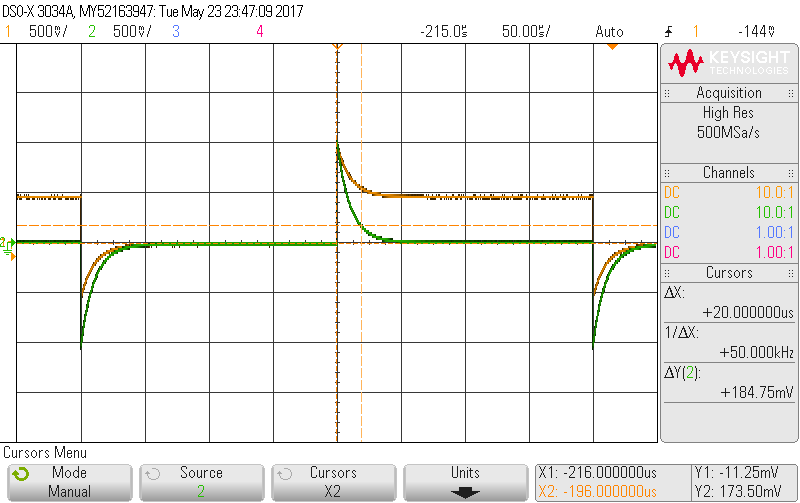
\includegraphics[width=100mm]{sprungantwort_rl_hochpass.png}
  \caption{Sprungantwort RL Hochpass}
  \label{Figure07}
\end{figure}
\noindent Die Sprungantwort der RL-Filterschaltung l\"asst auf einen Hochpassfilter 1.Ordnung schlie\ss en, da bei niedriger Frequenz die D\"ampfung der Spannungsamplitude stark ist und bei hoher Frequenz auf $0 dB$ zur\"uck geht. Ein Hochpassfilter kann auch mit einem RC-Glied realisiert werden, wobei die Ausgangsspannung am Widerstand abgenommen wird.

\begin{figure}[H]
  \centering
  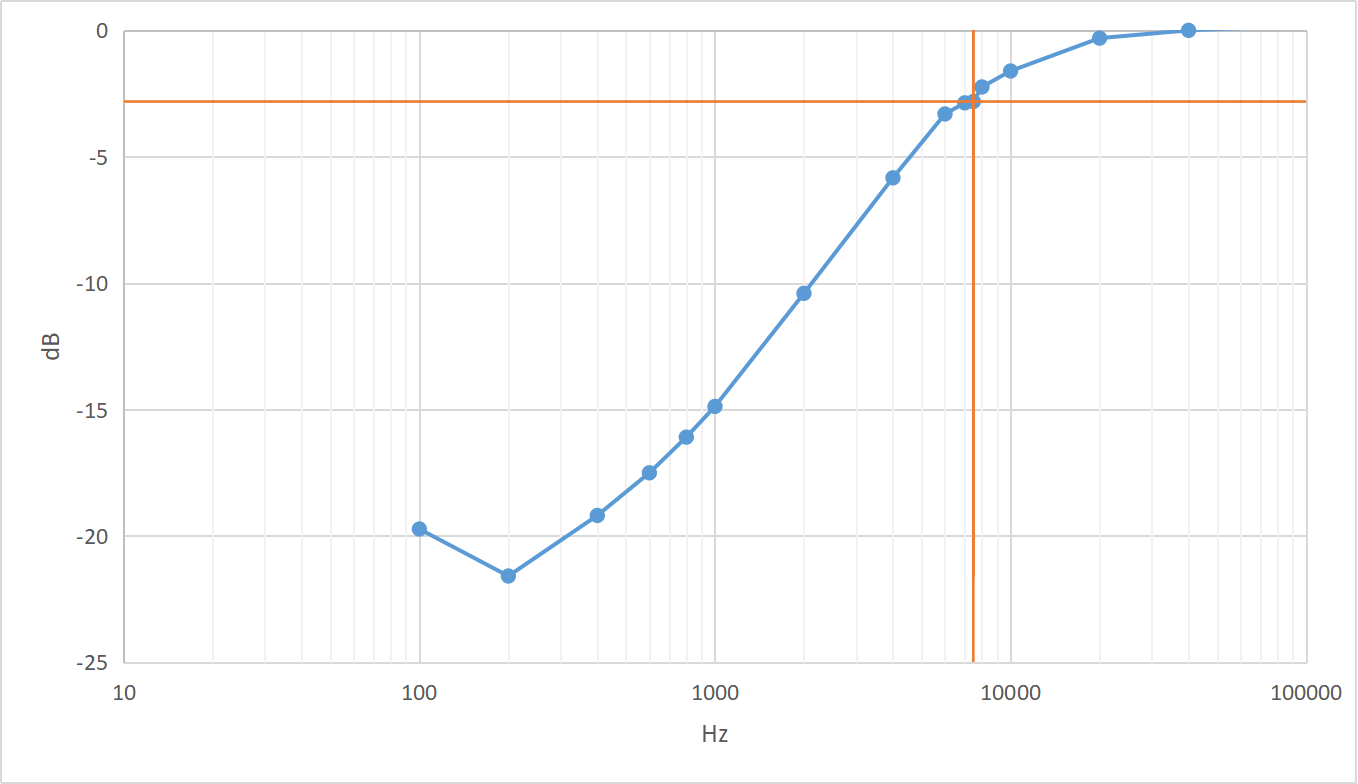
\includegraphics[width=100mm]{amplitudengang_rl_hochpass.png}
  \caption{Amplitudengang RL-Hochpass durch Messungen}
  \label{Figure08}
\end{figure}
\begin{figure}[H]
  \centering
  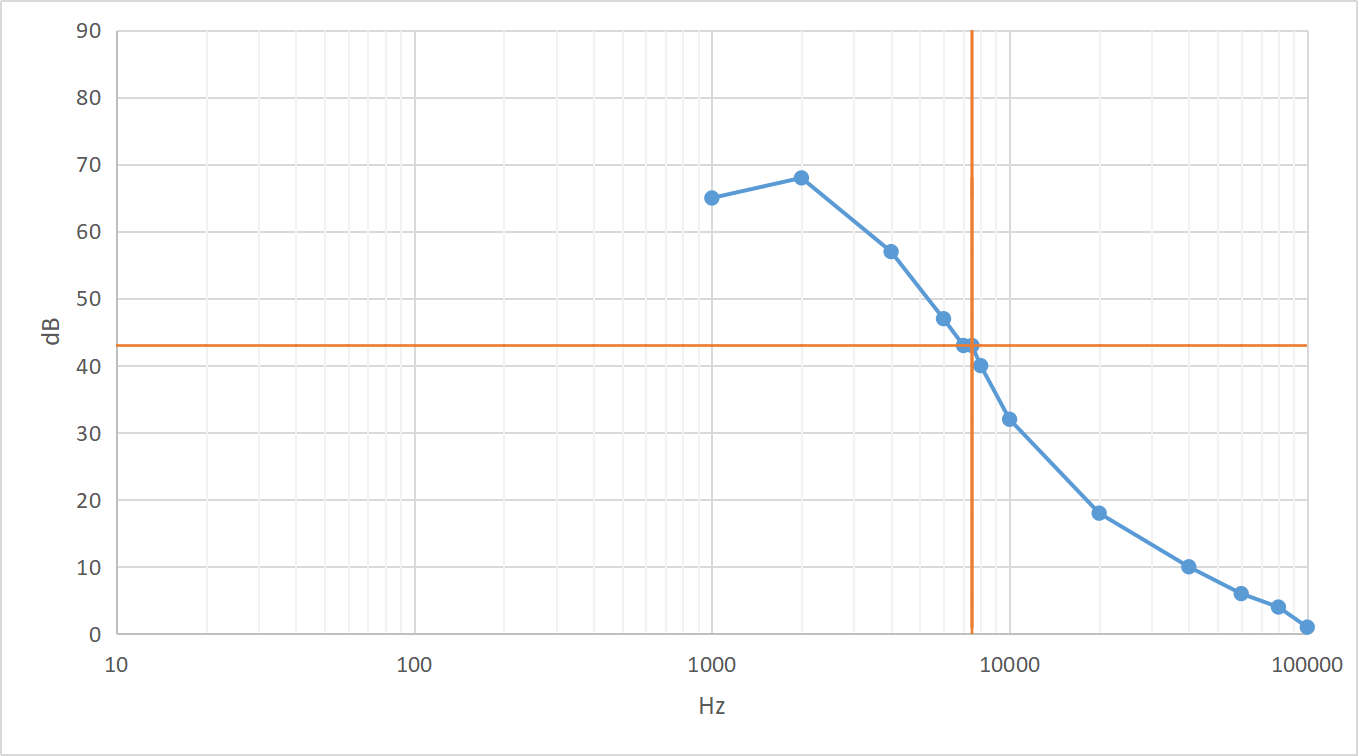
\includegraphics[width=100mm]{phasengang_rl_hochpass.png}
  \caption{Phasengang RL-Hochpass durch Messungen}
  \label{Figure09}
\end{figure}
In Abbildung~\ref{Figure07} sind Amplituden- und Phasengang des RL-Hochpassfilters anhand der gemessenen Werte dargestellt. Der Graph entspricht der erwarteten Form aus der Simulation. Die Eingangsspannung wird durch die Reflexion der Spule beeintr\"achtigt. Je h\"oher die Frequenz, desto st\"arker wurde die Verst\"arkung der Eingangsspannung. Bis zur Frequenz von $1 kHz$ konnte kaum eine Ver\"anderung festgestellt werden, bei der Frequenz von $60 kHz$ war die gemessene Eingangsspannung bereits doppelt so gro\ss. Das Verh\"ahtnis von Eingangs- und Ausgangsspannung verhielt sich jedoch wie in der Simulation. Bei der Grenzfrequenz ($7480$) wurde am Eingang $U_e = 650mV$, am Ausgang $U_a = 470mV$ und eine Phasenverschiebung von $43^{\circ}$ gemessen.






\section{Messung des Verhaltens eines dynamischen Systems 2. Ordnung}

\subsection{Aufgabenstellung}
Die Sprungantwort sowie das Frequenzverhalten eines RLC-Systems 2. Ordnung soll untersucht werden.

\subsection{Schaltplan}
\begin{figure}[H]
  \centering
  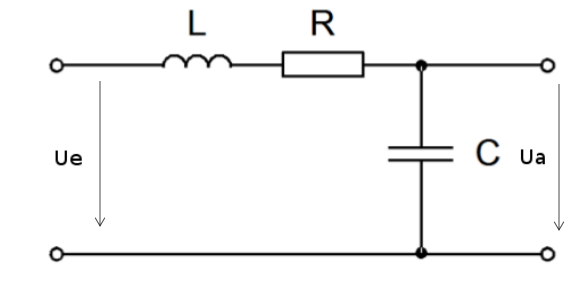
\includegraphics[width=100mm]{rlc_schaltplan.png}
  \caption{RLC-System 2.Ordnung}
\end{figure}

\subsection{Durchf\"uhrung}
Die Schaltung wurde gem\"aß Schaltplan mit den Bauteilwerten $L=1mH$, $C=100nF$ und $R=22\Omega$ aufgebaut. Um die Sprungantwort des Systems mit dem Oszilloskop aufzuzeichnen, wurde als Eingangssignal eine periodische Rechteckschwingung mit $1Vpp$, Offset $0,5V$ und Frequenz $2,5kHz$ (Periodendauer $400\mu s$) angelegt. Weiters wurde das Frequenz- bzw. D\"ampfungsverhalten des Systems mit einem Sinussignal ($1Vpp$) ermittelt. Hierbei wurde zuerst die Resonanzfrequenz durch Variation der Frequenz des Eingangssignals bestimmt. Diese ist erreicht, wenn Eingangs- und Aussgangsignal eine Phasenverschiebung von $-90^{\circ}$ zueinander aufweisen. Um den Amplitudengang des Systems zu ermitteln, wurden Eingangs- und Ausgangspannung an verschiedenen Frequenzmesspunkten im lograithmischen Maßstab ermittelt. Im Bereich der Resonanzfrequenz wurden zusätzlich Messpunkte gewählt, um die Genauigkeit zu erhöhen. Die oben beschriebene Vorgangsweise wurde mit den Widerstandswerten $R = 183 \Omega$ (in der Angabe wurden $180\Omega$ verlangt, es gibt jedoch keinen Normwiderstand mit diesem Wert, darum wurden hier ein $150\Omega$ und ein $33\Omega$ in Serie geschalten) und $R = 1k\Omega$ wiederholt.

\subsection{Ergebnis \& Diskussion}
Die Resonanzfrequenz des Systems ergibt sich aus folgender Formel:
\begin{figure}[H]
  \centering
  $f_R = \sqrt{f_H*f_L} = \frac{1}{2\pi\sqrt{LC}} \approx 15916Hz$
\end{figure}

\begin{figure}[H]
  \centering
  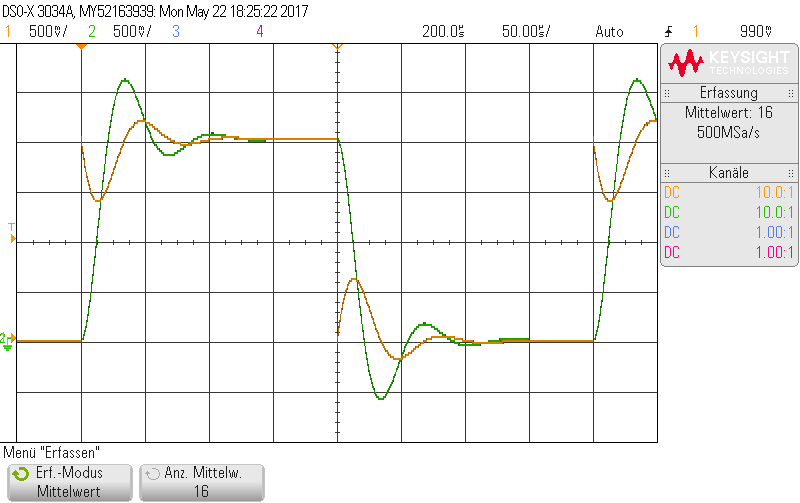
\includegraphics[width=100mm]{sprungantwort_rlc_22.png}
  \caption{Sprungantwort bei $R=22\Omega$}
\end{figure}
Durch den kleinen Widerstand ($R=22\Omega$) ist die Dämpfung des Systems sehr gering und es wird auch das Schwingungsverhalten des $LC$-Glieds deutlich sichtbar (\"Uberschwingung). Verursacht durch die parasit\"aren Eigenschaften der realen Bauelemente kommt es zu Effekten, die sich auf die Eingansspannung auswirken.

\begin{figure}[H]
  \centering
  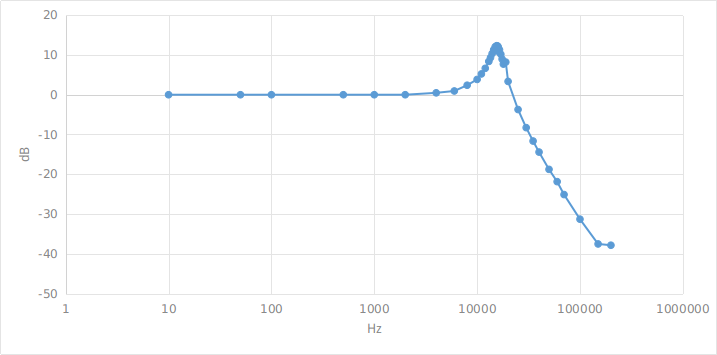
\includegraphics[width=150mm]{bode_rlc_22.png}
  \caption{Bode-Diagramm (Amplitudengang) bei $R=22\Omega$}
\end{figure}
\noindent Die gemessene Resonanzfrequenz betr\"agt hier $\sim15,8kHz$ (Abweichung $-0,7\%$). Im Bereich von $f_R$ erkennt man am Bode-Diagramm, dass hier tats\"achlich eine Verstärkung des Eingangsignals stattfindet. Dies lässt sich durch die kleine Dämpfung bei $R=22\Omega$ erkl\"aren, wodurch sich das $LC$-Glied im Resonanzfall befindet. Nach dem die Resonanzfrequenz erreicht wurde, lässt sich die typische Filtersteilheilt von $-40dB/Dekade$ gut erkennen.\\

\begin{figure}[H]
  \centering
  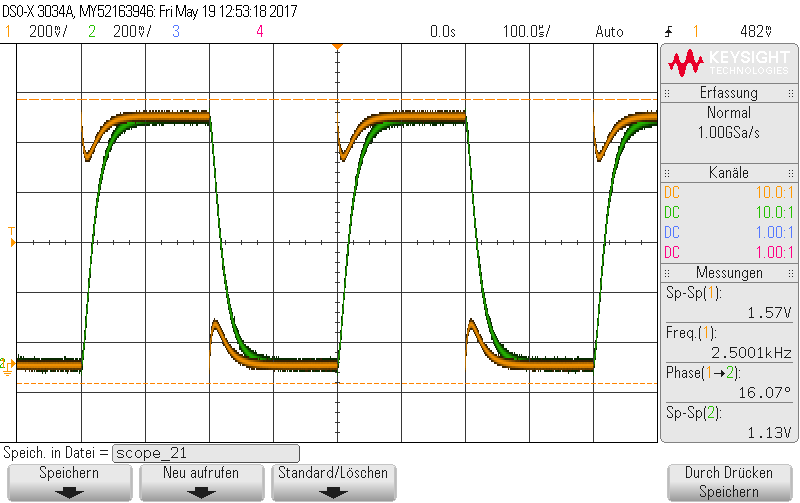
\includegraphics[width=100mm]{sprungantwort_rlc_180.png}
  \caption{Sprungantwort bei $R=183\Omega$}
\end{figure}
\noindent Bei $R=183\Omega$ sind gerade keine \"Uberschwingungen sichtbar (aperiodischer Grenzfall). Die Sprungantwort zeigt das typische Tiefpassverhalten.

\begin{figure}[H]
  \centering
  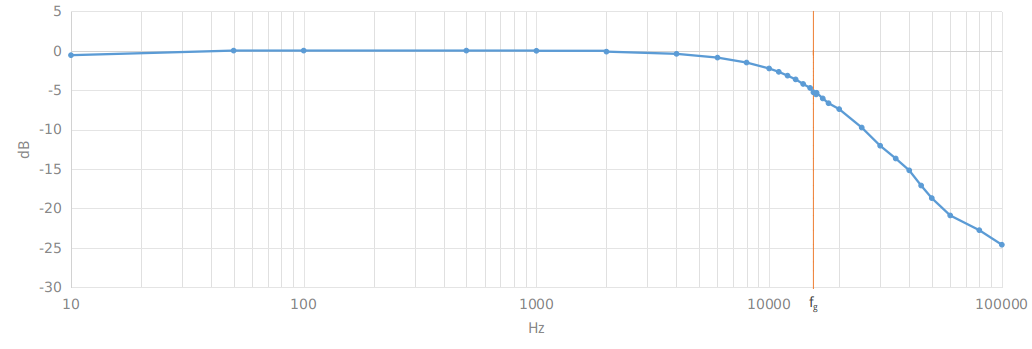
\includegraphics[width=150mm]{bode_rlc_180.png}
  \caption{Bode-Diagramm (Amplitudengang) bei $R=183\Omega$}
\end{figure}
\noindent Die gemessene Resonanzfrequenz betr\"agt hier $\sim15,5kHz$ (Abweichung $-2,61\%$). Das System befindet sich im aperiodischen Grenzfall. Auch hier lässt sich die typische Filtersteilheit von $-40dB/Dekade$ aus dem Diagramm ablesen.\\

\begin{figure}[H]
  \centering
  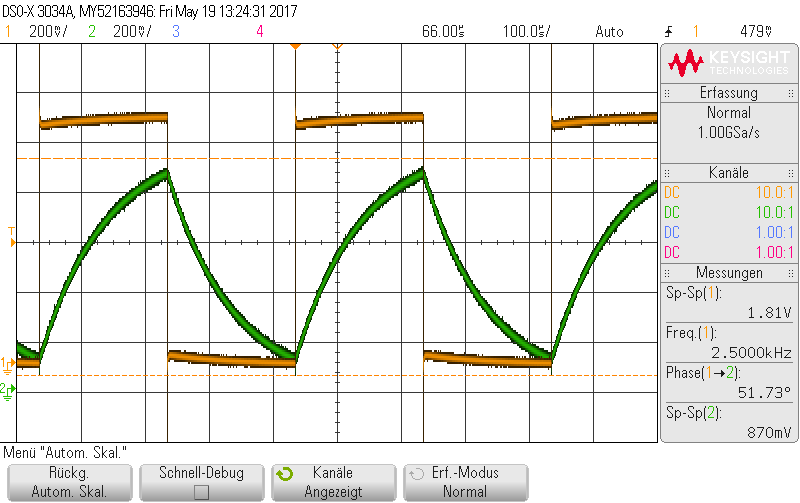
\includegraphics[width=100mm]{sprungantwort_rlc_1k.png}
  \caption{Sprungantwort bei $R=1k\Omega$}
\end{figure}
\noindent Durch den großen Widerstand von $R=1k\Omega$ wird die D\"ampfung des Systems sehr groß. Dadurch wird in der Folge die anliegende Rechteckspannung stark verschliffen.

\begin{figure}[H]
  \centering
  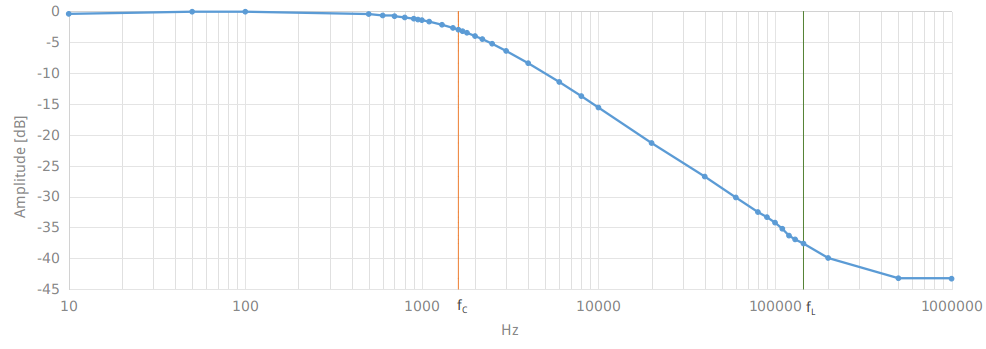
\includegraphics[width=150mm]{bode_rlc_1k.png}
  \caption{Bode-Diagramm (Amplitudengang) bei $R=1k\Omega$}
\end{figure}
\noindent Durch den großen Widerstand wird die Grenzfrequenz des Kondensators $f_C$ (orange) früher erreicht, sie liegt laut Messung bei $\sim1,6kHz$. Die Grenzfrequenz der Spule $f_L$ (gr\"un) wird laut Messung erst bei $\sim145kHz$ erreicht. Nachteilig ist hier, dass im Bereich zwischen $f_C$ und $f_L$ nur eine Filtersteilheit von $-20dB/Dekade$ erreicht wird.\\\\

\noindent Der Widerstand hat aus rein mathematischer Sicht keinen Einfluss auf die Resonanzfrequenz, wie man an obenstehender Formel sehen kann. Bei den Messungen zeigen sich jedoch leichte Abweichungen von der berechneten Resonanzfrequenz, dies sind auf die Eigenschaften realer Bauteile zurückzuführen.\\\\

\noindent Im Vergleich zu den Simulationen lässt sich sagen, dass das simulierte Verhalten des Filters mit verschiedenen Widerständen im Labor sehr gut messbar und nachvollziehbar war. Es zeigen sich jedoch einige Ungenauigkeiten, die auf reale Bauteile und Messfehler zurückzuführen sind.\\\\

\noindent Die \"Ubertragungsfunktion des Systems lautet:
\begin{figure}[H]
  \centering
  $\frac{U_a}{U_e} = \frac{Z_C}{Z_R+Z_L+Z_C} = \frac{\frac{1}{j\omega C}}{R+j\omega L+\frac{1}{j\omega C}} = \frac{1}{j\omega CR-\omega^2CL+1} = \frac{1}{s^2CL+sCR+1}$
\end{figure}


\begin{figure}[H]
  \centering
  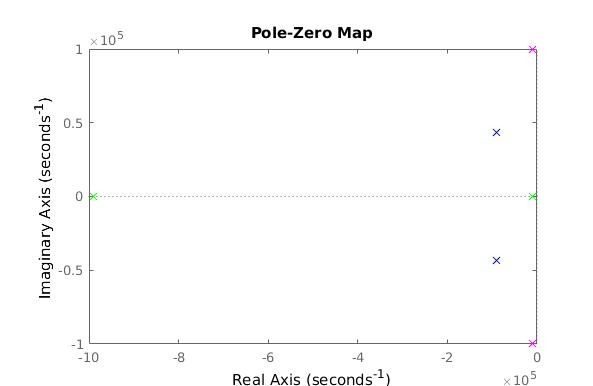
\includegraphics[width=150mm]{pnd.jpg}
  \caption{PN-Diagramm der \"Ubertragungsfunktion (violett: $R=22\Omega$, blau: $R=180\Omega$, gr\"un: $R=1k\Omega$)}
\end{figure}

\end{document}
